\chapter{Results - Sliding Puzzle} % Main chapter title

\label{sec:ResultsSP} % Change X to a consecutive number; for referencing this chapter elsewhere, use \ref{ChapterX}


In this chapter, I show and discuss results on \textbf{SP} of various dimensions, going from \textit{small} dimensions (which I define as those I can reasonably \textit{fully} solve given my computing resources, the finite time I have to complete this project, and the choice of programming language), then I move to studying in much detail the case of the 3x3, and finally move on to slightly higher dimensions 3x4 and 4x4. Table \ref{tab:gridSP} below shows which solvers I have run on each of the dimensions attempted. The reader is referred to the implementation chapter \ref{sec:Implementation} for a detailed explanation of each of these solvers, and to the appendix section \ref{sec:Examples} for code examples on how to run them.

\begin{table}[H]
\begin{center}
\begin{tabular}{l*{9}{c}r}
\hline
\textbf{solver}      & & \textbf{Sliding Puzzle} & \textbf{2x2} & \textbf{2x3} & \textbf{2x4} & \textbf{2x5}  & \textbf{3x3} & \textbf{3x4} & \textbf{4x4} \\ 
\hline
BFS   & & & & & & &  x  & & \\
\hline
A$^{*}$[Manhattan]   & & & & & &  x  &  x  &  x  & \\
\hline
A$^{*}$[Manhattan++]   & & & & & &  x  &  x  &  x  & x \\
\hline
A$^{*}$[Perfect]   & & &  x  &  x  &  x  &  x  &  x  & & \\
\hline
Naive   & & & & & & &  x  &  x  & x \\
\hline
A$^{*}$[DL[FullyConnected]]   & & & & & & &  x  &  x  & x \\
\hline
A$^{*}$[DL[Convolutional]]   & & & & & & &  x  &  & \\
\hline
A$^{*}$[DRL]   & & & & & & &  x  &  x  & x \\
\hline
A$^{*}$[DQL]   & & & & & & &  x  & & \\
\hline
MCTS[DQL]        & & & & & & &  x  & & \\
\end{tabular}
\caption{\label{tab:gridSP} Solvers used vs \textbf{SP} dimension}
\end{center}
\end{table}

I am neither making claims of depth (each solver could surely be tuned and optimized/adapted, possibly differently for each dimension) nor breadth (I have not run all of the solvers versus each dimension). Running these experiments takes a lot of time, so I had to be somewhat selective. I wanted however to run all of the solvers I have implemented one particular dimension (the intermediary 3x3 seemed appropriate to do so), to answer some of the following interesting questions:
\begin{itemize}
\item How hard is too hard for \textbf{BFS} to complete in \textit{reasonable} time?
\item How much, if any, improvement do we get with Manhattan++ over Manhattan?
\item Is there much loss between \textbf{DL} and \textbf{DRL}, i.e. is losing the teacher used by \textbf{DL} a deal breaker?
\item Is \textbf{DQL}, all things being equal, able to learn a better cost-to-go heuristic than \textbf{DRL}?
\item How does \textbf{MCTS} perform? How important is it to tune the hyper-parameter $c$? How much improvement, if any, does the post trim of the \textbf{MCTS} tree via \textbf{BFS} bring?
\item Are any of the \textbf{D*L} techniques able to perform on par with A$^{*}$ with Manhattan++ or perfect heuristic?
\end{itemize}
All of these questions are answered (obviously not in generality, but in the context of the experiments I have been running) in this chapter.











%----------------------------------------------------------------------------------------
%	SECTION 1
%----------------------------------------------------------------------------------------

\section{Low dimension}
\label{sec:SPLowDimension}

\subsection{God numbers and hardest puzzles}

As mentioned in chapter \ref{sec:Puzzles}, the state space cardinality for the SP grows very quickly with n and m. The only dimensions which have less than 239.5 millions states are shown in table \ref{tab:smallSP}. Note I am also only considering n $\leq$ m since dimension (m, n) can always be solved by symmetry from the solutions (n, m):

\begin{table}[H]
\begin{center}
\begin{tabular}{l*{6}{c}r}
n              & m & 2 & 3 & 4 & 5\\
\hline
2              &   & 12 & 360 & 20,160 & 1,814,400 \\
3              &   &   & 181,440 &  &    \\
\end{tabular}
\caption{\label{tab:smallSP}\# puzzles for \textit{small} dimensions}
\end{center}
\end{table}
In this section, I will discuss \textit{full} results for these 5 dimensions. In order to fully solve them, one can simply use rubiks.scripts.learner, setting up the PerfectLearner with A* and manhattan heuristic, or instantiate directly a PerfectLearner as have seen in section \ref{PLSS}. I obtained the following God numbers (table \ref{tab:smallSPGN}) for these puzzles:
\begin{table}[H]
\begin{center}
\begin{tabular}{l*{6}{c}r}
n              & m & 2 & 3 & 4 & 5\\
\hline
2              &   & 6 & 21 & 36 & 55* \\
3              &   &   & 31 &  &    \\
* \tiny{provisional result}
\end{tabular}
\caption{\label{tab:smallSPGN}God numbers for \textit{small} dimensions}
\end{center}
\end{table}
Notice that among the above dimensions, (n=2, m=5) is the largest and hardest one. I had to run its PerfectLearner over a many weeks (whenever I had spare computing capacity and over a full week-end on a c5.18xlarge instance (72 cores) on Amazon EC2).
\\
\\
The perfectLearner also keeps track of the hardest puzzle it has encountered (i.e. a configuration whose optimal solution has a cost equal to the God number). I obtained the following hardest puzzles for each of the 5 \textit{small} dimensions:
\\
\\
\underline{Most difficult 2x2 (6 moves)}:
\begin{center}
\begin{three}
\setrow{2}{,3}
\setrow{1}{2,1}
\end{three}
\end{center}
\underline{Most difficult 2x3 (21 moves)}:
\begin{center}
\begin{five}
\setrow{2}{4,5,}
\setrow{1}{1,2,3}
\end{five}
\end{center}
\underline{Most difficult 2x4 (36 moves)}:
\begin{center}
\begin{seven}
\setrow{2}{,7,2,1}
\setrow{1}{4,3,6,5}
\end{seven}
\end{center}
\underline{Most difficult 2x5 (55* moves)}:
\begin{center}
\begin{nine}
\setrow{2}{,9,3,7,1}
\setrow{1}{5,4,8,2,6}
\tiny{* provisional result}
\end{nine}
\end{center}
\underline{Most difficult 3x3 (31 moves)}:
\begin{center}
\begin{eight}
\setrow{3}{8,6,7}
\setrow{2}{2,5,4}
\setrow{1}{3,,1}
\end{eight}
\end{center}




\subsection{Manhattan heuristic}
\label{MHComp}
In this section, I verify empirically that, as expected, the overhead of adding penalty in Manhattan++ for the linear constraint (which have all been precomputed and stored in a database) is more than compensated for by the reduction in nodes expansion. I have run my solver script for (n=2, m=5) in performance test mode, for both Manhattan and Manhattan++, with 250 randomly shuffled puzzles with \textit{nb\_shuffles} from 0 to 60 by increment of 5, as well as with \textit{nb\_shuffles = $\inf$}. The resulting run time and nodes expansions are as follows:

\begin{figure}[H]
\centering
%\hspace*{-2.5cm}
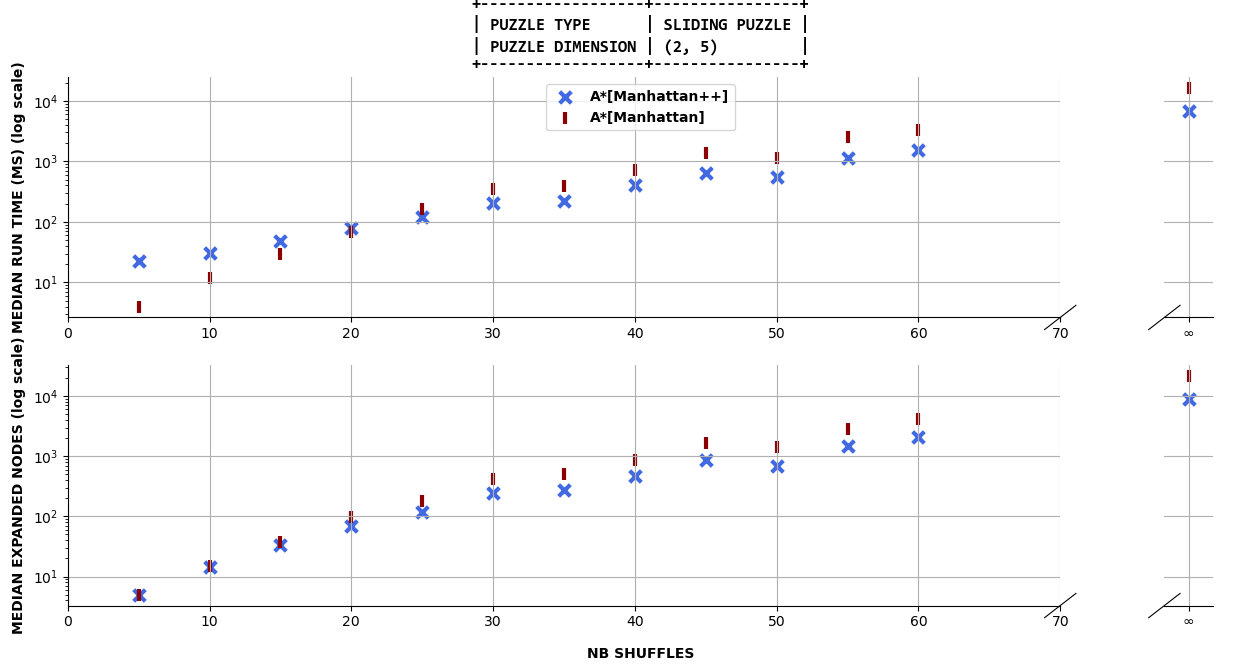
\includegraphics[scale=0.40]{./Figures/25SPPerformanceManhattan}
%\decoRule
\caption[SP]{Manhattan vs Manhattan++ for the 2x5 \textbf{SP}}
\label{fig:25SPPerformanceManhattan}
\end{figure}

As can be seen, for low difficulty (up to \textit{nb\_shuffles = 20}), the node expansions are about the same in both cases, and the overhead of adding the linear constraints penalty increases the run time. However, for any non trivial case, Manhattan++ outperforms considerably (by a factor of about 2.5). Table \ref{tab:mppOutperformance} below summarizes the results for the 250 \textit{perfectly} shuffled instances:



\begin{table}[H]
\begin{center}
\begin{tabular}{l*{7}{c}r}
                              & avg cost  & max cost & avg nodes & max nodes & avg run time (ms) & max run time (ms) \\
\hline
Manhattan                   &  34.6  & 49 & 46,483 & 575,050 & 36,088 & 428,887 \\
Manhattan++              & 34.6 &  49 & 18,780 & 213,557 & 14,665 & 165,830 \\
Improvement               & n/a &  n/a & x2.5 & x2.7 & x2.5 & x2.6 \\
\end{tabular}
\caption{\label{tab:mppOutperformance} Manhattan++ outperformance on perfectly scrambled 2x5 \textbf{SP}}
\end{center}
\end{table}






%-----------------------------------
%	SECTION 2
%-----------------------------------
\section{Intermediary case - 3x3}
\label{sec:S33}


\subsection{Perfect learner}
As discussed in the previous section section \ref{sec:SPLowDimension}, the 3x3 \textbf{SP} is one of the cases I have been able to solve perfectly, since it only has 181,440 possible configurations. Its God number is only 31, which definitely makes it manageable. However, this is already an intermediary size, large enough that it is worth trying and comparing a few different methods, including deep reinforcement learning. To start with, I ran the PerfectLearner with n=m=3, and the results are shown below in figure \ref{fig:33SPPerfectLearning}. It is interesting to note that there are only two hardest configurations (cost 31) and 221 configurations of cost 30.


\begin{figure}[H]
\centering
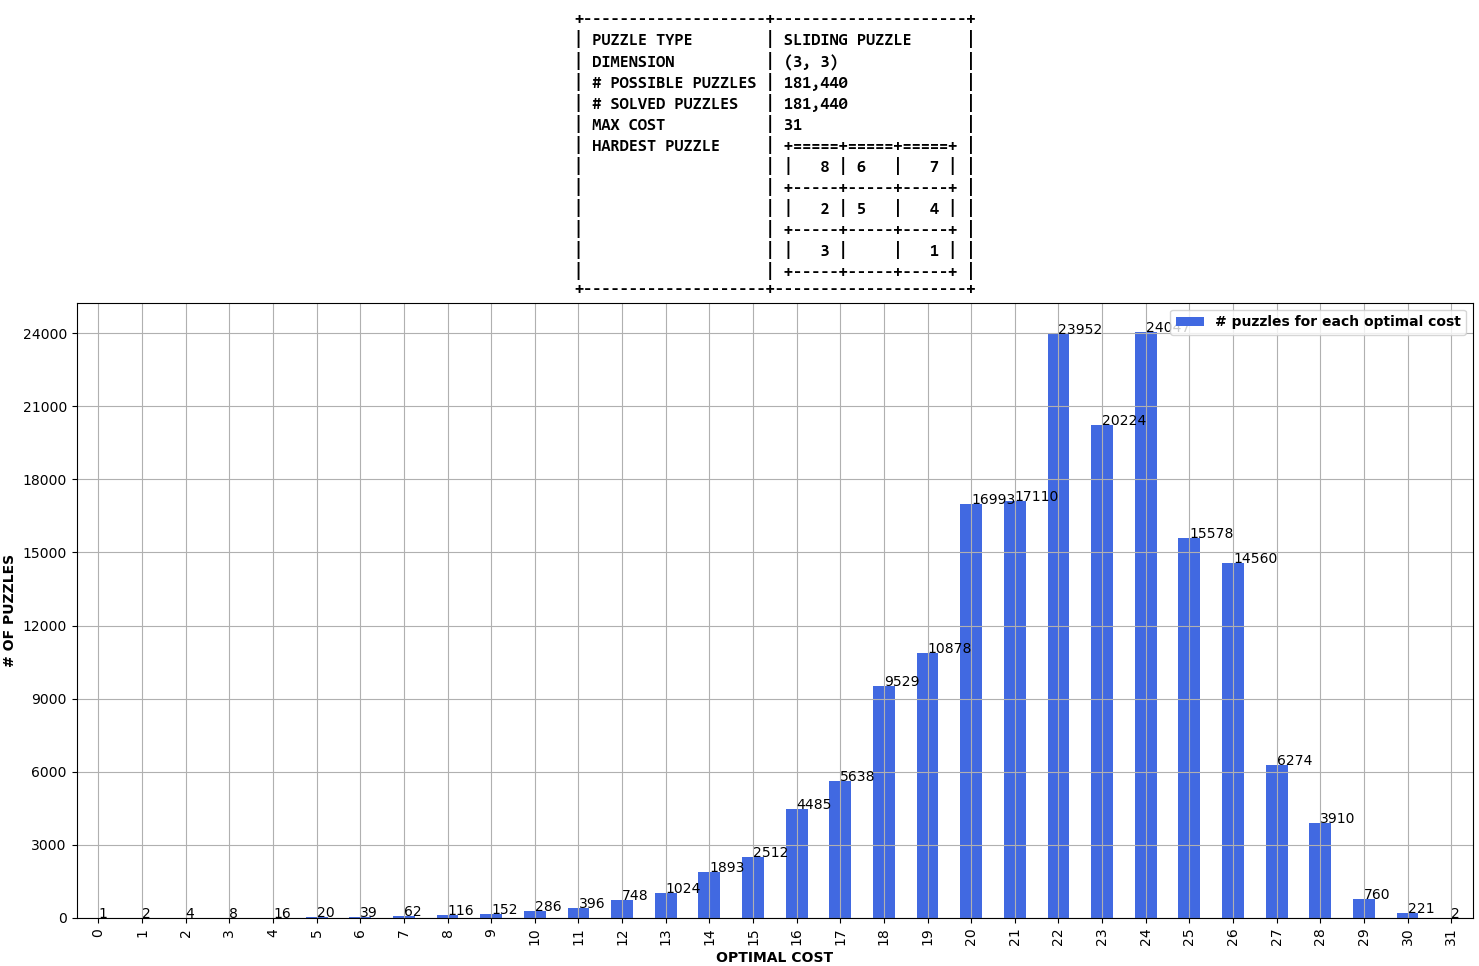
\includegraphics[scale=0.42]{./Figures/33SPPerfectLearning}
\caption[33SPPerfectLearning]{Perfect Learning of the 3x3 \textbf{SP}}
\label{fig:33SPPerfectLearning}
\end{figure}




\subsection{Deep reinforcement learner}
 The DeepReinforcementLearner's learning is shown in figure \ref{fig:33SPDeepReinforcementLearning}:

\begin{figure}[H]
\centering
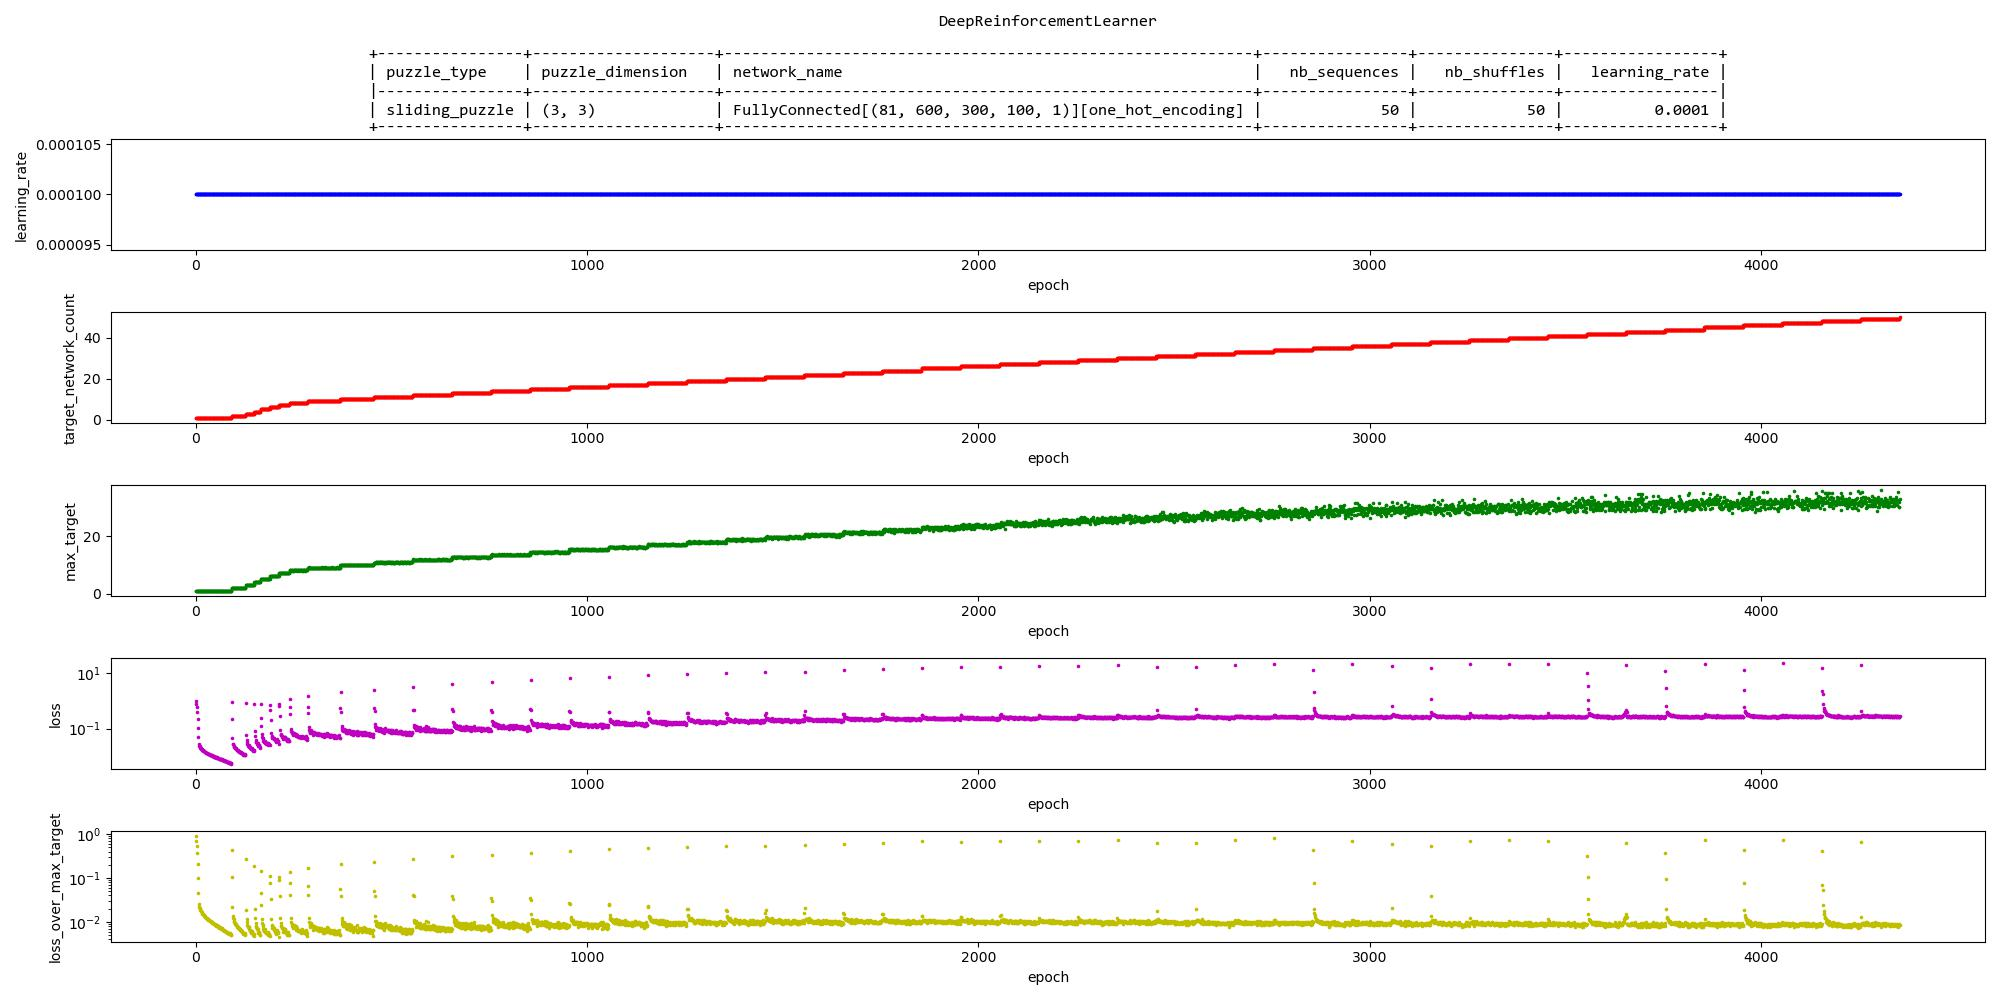
\includegraphics[align=c, scale=0.42]{./Figures/33SPDeepReinforcementLearning}
\caption[33SPDeepReinforcementLearning]{\textbf{DRL} of the 3x3 \textbf{SP}}
\label{fig:33SPDeepReinforcementLearning}
\end{figure}


\subsection{MCTS DQL}
\label{sec:MTCSHyperParamsEffect}


\begin{figure}[H]
\centering
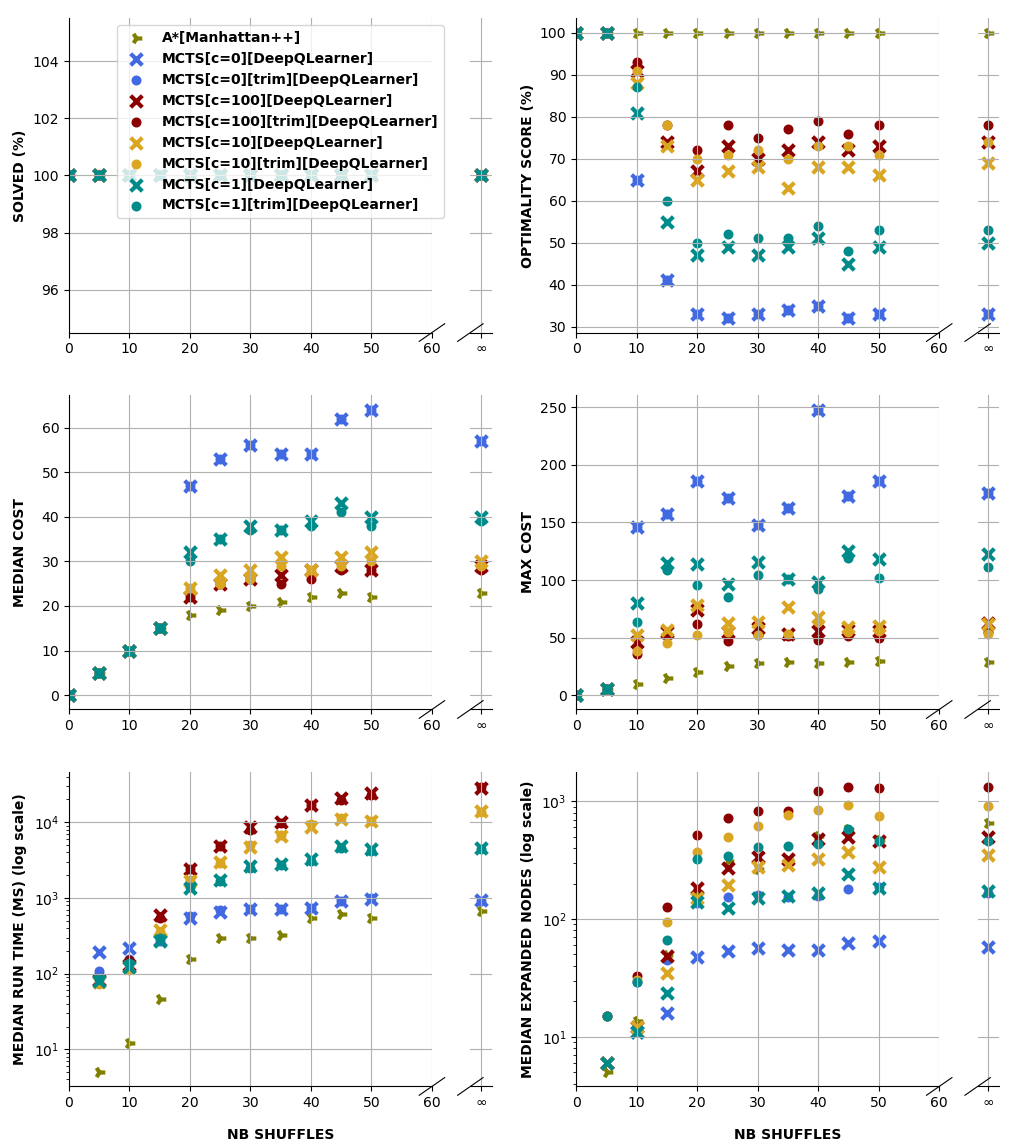
\includegraphics[align=c, scale=0.6]{./Figures/33SPPerformanceMCTS}
\caption[33SPPerformanceMCTS]{\textbf{MCTS} tuning 3x3 \textbf{SP}}
\label{fig:33SPPerformanceMCTS}
\end{figure}



\subsection{Solvers' comparison}
\label{ssec:33SPSC}
\label{sec:S33DRLDQL}
Let me discuss a comparison of several algorithms on 1000 random puzzles generated for a number of random shuffling (with best-effort-no-backtracking) from 0 to 50 in step of 2, as well as for perfect shuffling (denoted by $\infty$) on the comparison graphs. The results are shown in figure \ref{fig:33SPPerformance}
\\
DL: 100 seq 15 to 31 shuffles 10k epochs connected 600 300 100
\\
Manhattan vs ++
\\
DQL vs DRL
\\
DxL vs Perfect
\\ Put table for nb\_shuffle=inf and highlight best in diff categories (cost, optimality score, run time, nodes)
\\ say how much of the puzzles the solvers have seen



\begin{figure}[H]
\centering
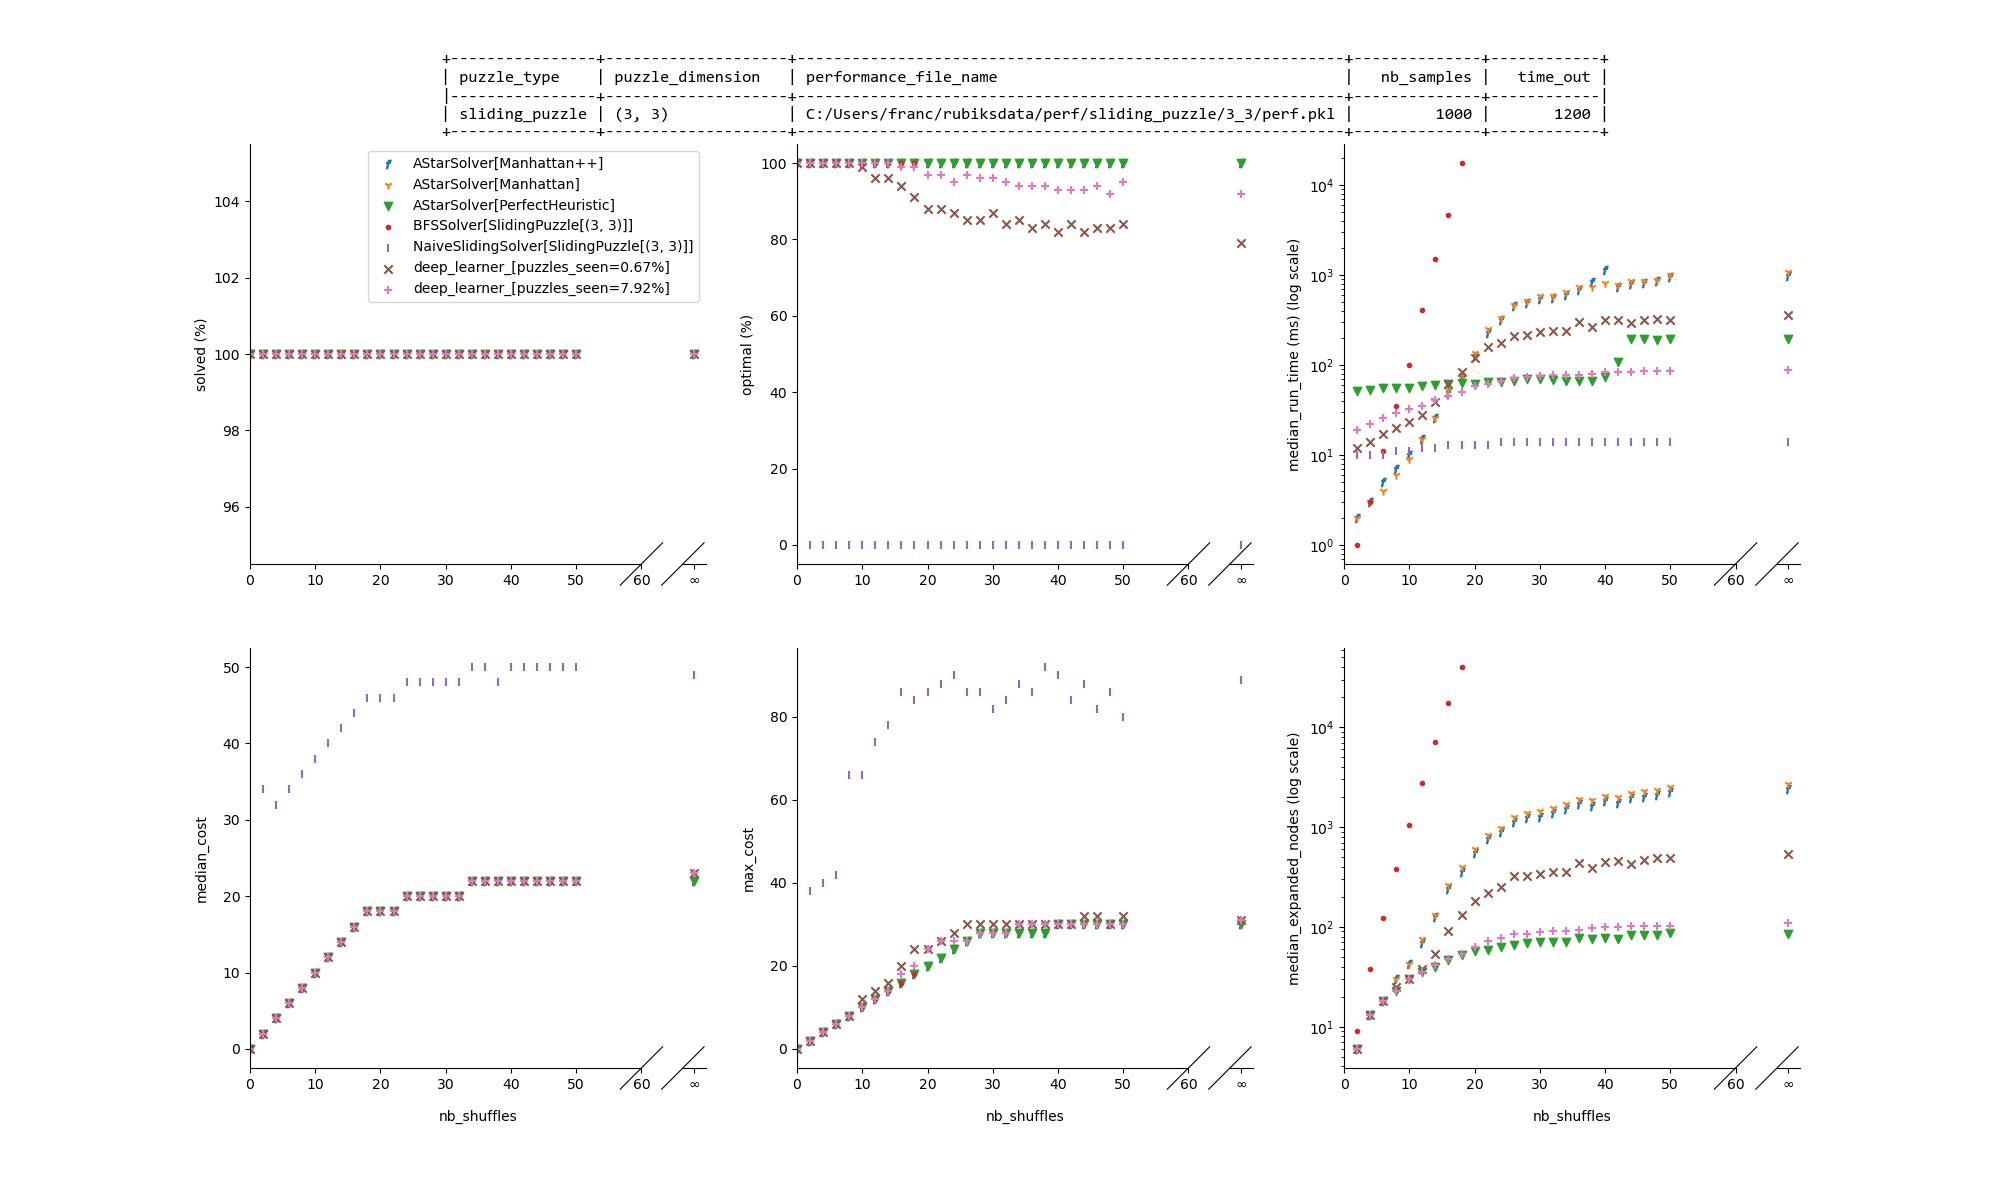
\includegraphics[scale=0.65]{./Figures/33SPPerformance}
%\decoRule
\caption[33SPPerformance]{Solvers' performance comparison 3x3 \textbf{SP}}
\label{fig:33SPPerformance}
\end{figure}


\subsection{Solving the hardest 3x3 problem}
To finish with the 3x3 SP, let me try to throw one of the two hardest 3x3 configurations (see subsection \ref{sec:SPLowDimension}) at the different solvers to see how they fare. The results are shown here

\begin{center}
\begin{tabular}{l*{5}{c}r}
\hline
\textbf{solver}      & & \textbf{cost} & \textbf{\# expanded nodes} & \textbf{run time (ms)} \\
\hline
AStarSolver[Manhattan]   &   &      31  & 58,859  & 11,327  \\
\hline
AStarSolver[Manhattan++]   &   &      31  & 34,224  & 7,080  \\
\hline
AStarSolver[PerfectHeuristic]  &   & 31 & 1,585 & 202 \\
\hline
AStarSolver[DRLHeuristic]  &   & 31 & 101 & 58 \\
\hline
MCTSSolver[DQLHeuristic][c=0]  &   & 101 & 103 & 456 \\
\hline
MCTSSolver[DQLHeuristic][c=69]  &   & 35 & 2,244 & 8,873 \\
\hline
BFS  &   & - & - & time out \\
\hline
NaiveSlidingSolver  &   & 61 & n/a & 18 \\
\hline
\end{tabular}
\end{center}
On this specific configuration, \textbf{BFS} was unable to complete before the time-out of sixty seconds. In an implementation without duplicate pruning, \textbf{BFS} would time out no matter what the bound is set. Indeed, it would need to explore in the order of $3^{31}$ - roughly 617 trillions - nodes to reach the goal! Even with my implementation which does pruning, it would need to pretty much traverse the entire 3x3 \textbf{SP} tree.
\\
Rather interestingly, the \textbf{DRL} heuristic performs much better than the Manhattan heuristic (not super suprising), but also outperforms the perfect heuristic quite significantly both in terms of run time and of nodes expansion. Obviously there is no guarantee that the perfect heuristic will not be outperformed on some random configuration, and it does on this occasion. However, as we have seen in the previous subection \ref{ssec:33SPSC}, it is not the case on average.
\\
\textbf{MCTS} with $c$ = 0 performs rather poorly, finding the longest solution (even than my Naive solver). It does behave a bit like \textbf{DFS} when $c$ is very small, expect the direction of travel is a bit more informed. I increased $c$, and for values over 69, it always gave me a solution of cost 35, which is not bad at all.
\\
Finally, the naive solver outperforms every other solver in terms of run time, but finds a rather poor solution of 61 moves.



%-----------------------------------
%	SECTION 3
%-----------------------------------
\section{3x4}

\label{ssec:34SPSC}

\begin{figure}[H]
\centering
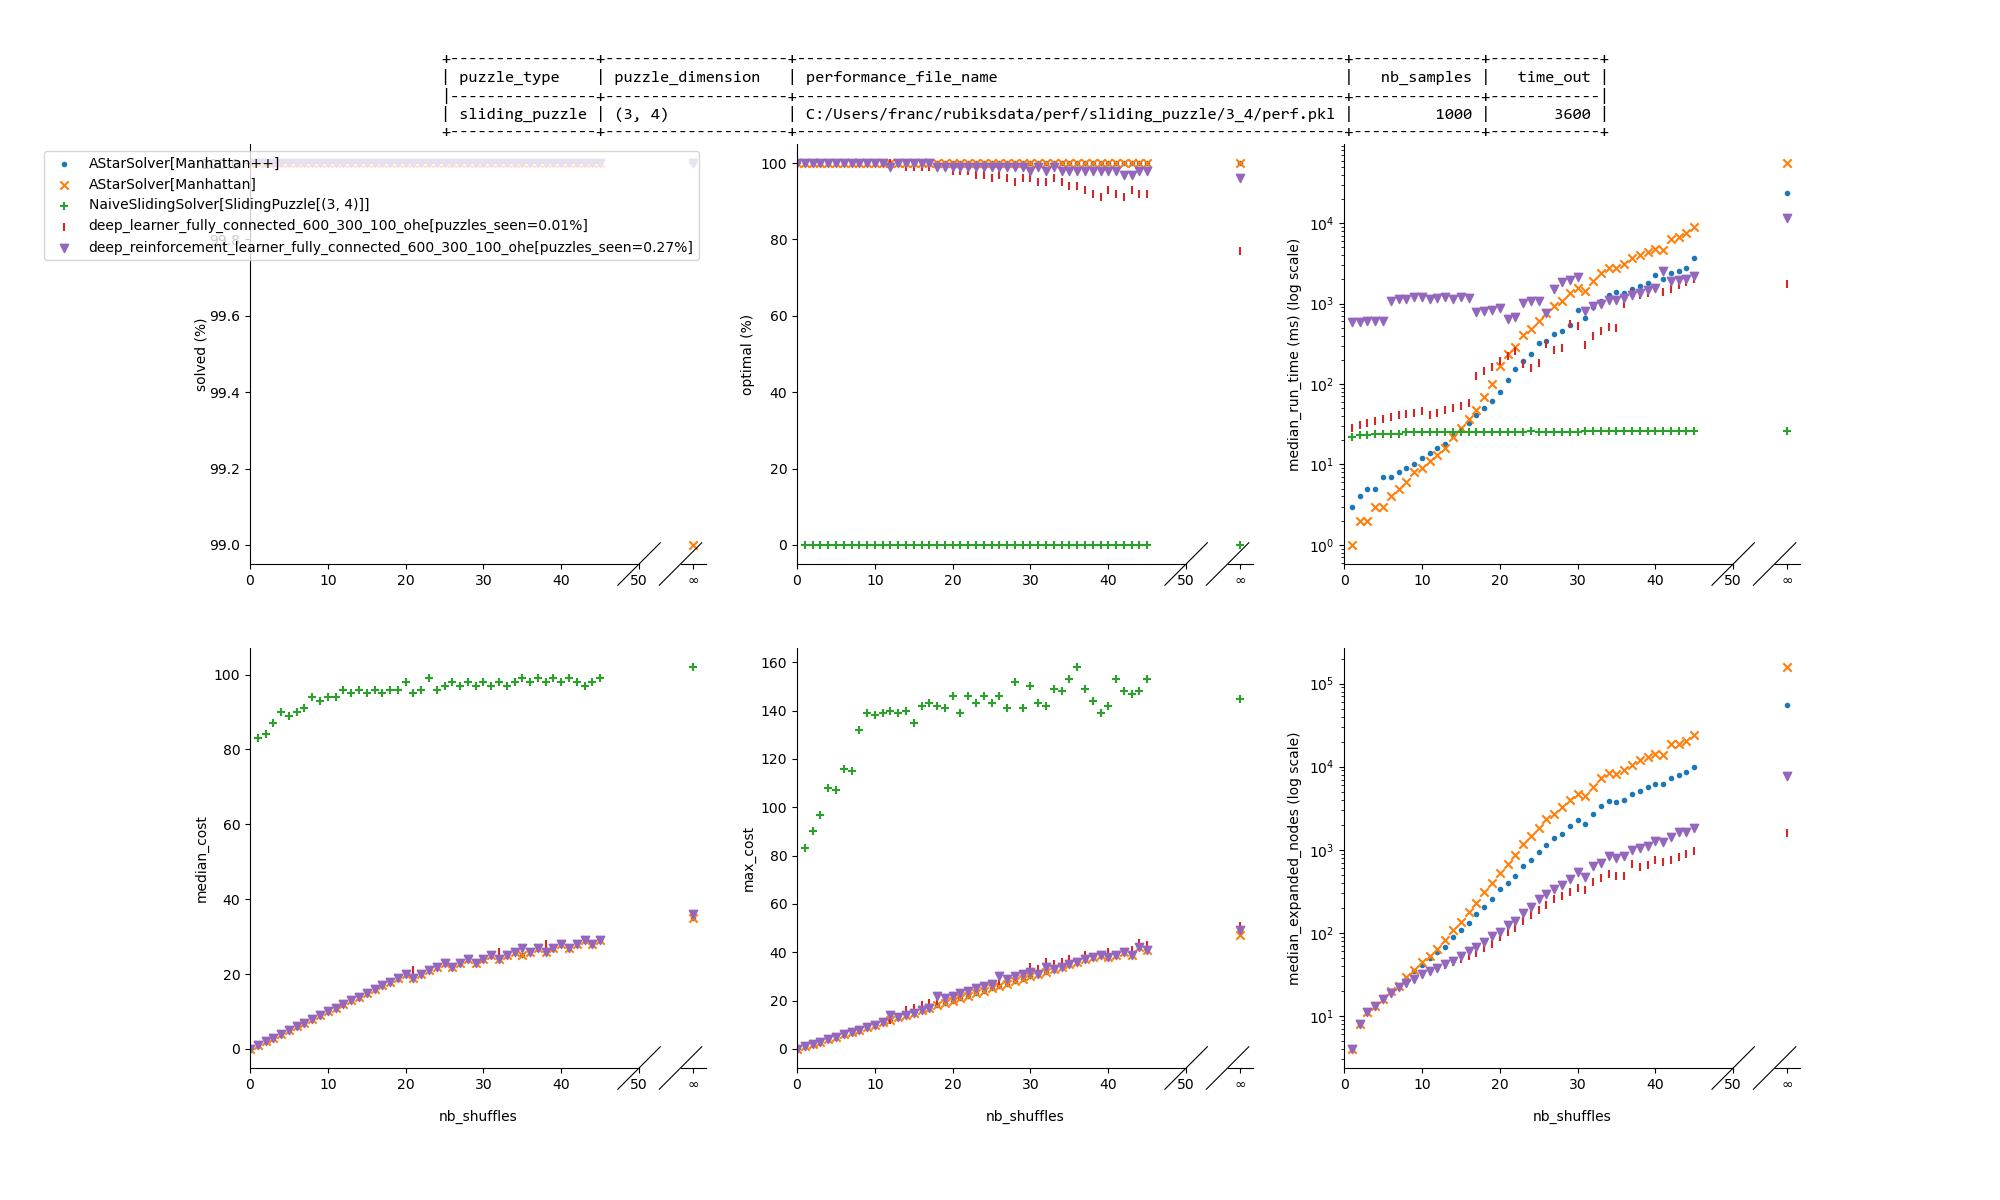
\includegraphics[scale=0.63]{./Figures/34SPPerformance}
%\decoRule
\caption[34SPPerformance]{Solvers' performance comparison 3x4 \textbf{SP}}
\label{fig:34SPPerformance}
\end{figure}





%-----------------------------------
%	SECTION 4
%-----------------------------------

\section{4x4}



\label{ssec:44SPSC}

\begin{figure}[H]
\centering
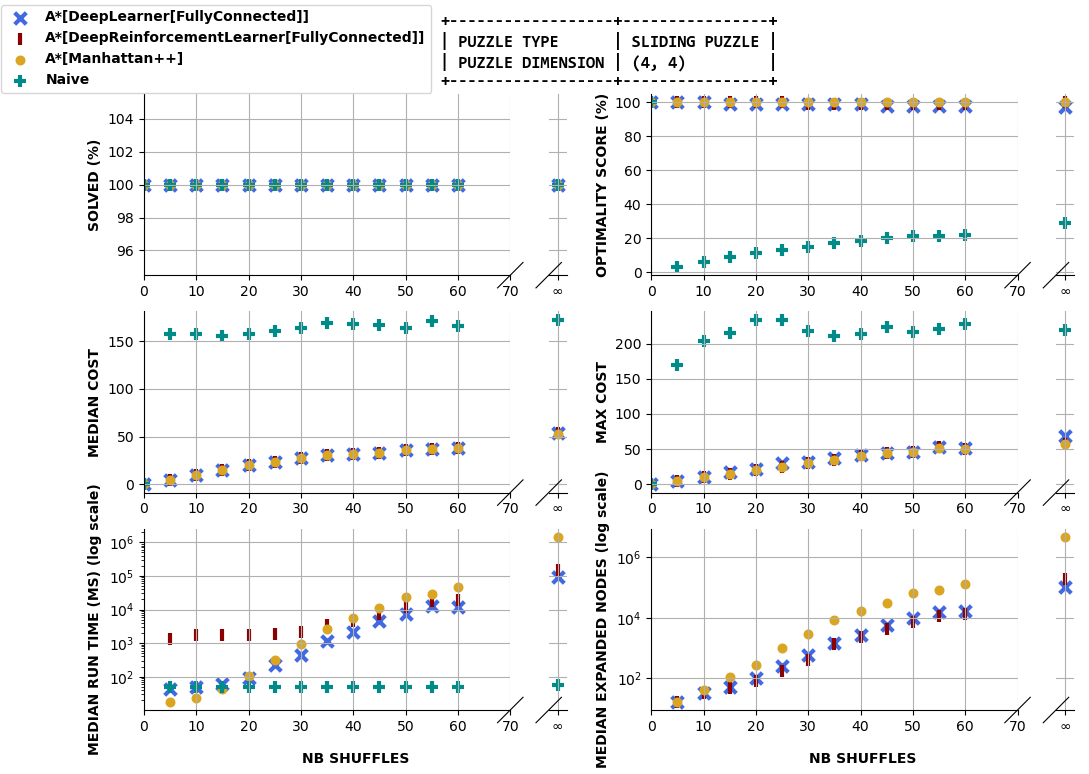
\includegraphics[scale=0.63]{./Figures/44SPPerformance}
%\decoRule
\caption[44SPPerformance]{Solvers' performance comparison 4x4 \textbf{SP}}
\label{fig:44SPPerformance}
\end{figure}

